% Source of the figure two-detours.pdf: the walk of the lemma on two detours. Highs are on the upper row and lows on the
% lower row of P. The red walk replaces the gray parts of P, which hold the positions of Z (here h and a).
% (a) a_2 at p_2 and b_1 at p_3. (b) a_2 at p_3 and b_1 at p_2, so the middle part is traversed backwards.
% Larger elements are drawn higher. Compile with pdfLaTeX; the PDF is included in the manuscript at its natural size.
\documentclass[tikz,border=1pt]{standalone}
\usepackage[T1]{fontenc}
\pdfinfoomitdate=1 \pdftrailerid{} \pdfsuppressptexinfo=-1
\definecolor{pathred}{RGB}{200,40,40}
\tikzset{
  vertex/.style={circle, fill=black, inner sep=0pt, minimum size=2.2mm},
  newvertex/.style={circle, fill=pathred, inner sep=0pt, minimum size=2.2mm},
  pathedge/.style={line width=1.8pt, pathred, line cap=round},
  oldedge/.style={line width=0.7pt, gray!80, dash pattern=on 3pt off 2pt}}
\newcommand{\zig}[3]{% from column #1 to column #2, style #3: odd columns are at height 1, even columns at height 0
  \foreach \c [evaluate=\c as \n using int(\c+1)] in {#1,...,\numexpr#2-1\relax} {
    \pgfmathsetmacro{\ya}{Mod(\c,2)}
    \pgfmathsetmacro{\yb}{Mod(\c+1,2)}
    \draw[#3] (\c,\ya) -- (\n,\yb);
  }}
\newcommand{\vertices}[1]{%
  \foreach \c in {1,3,...,#1} \node[vertex] at (\c,1) {};
  \foreach \c in {0,2,...,#1} \node[vertex] at (\c,0) {};}
\begin{document}
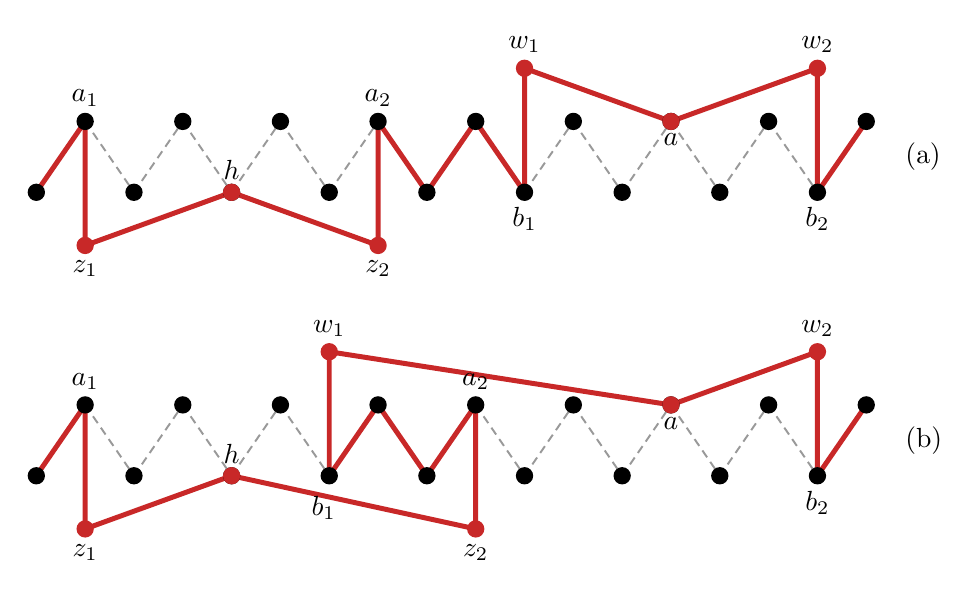
\begin{tikzpicture}[x=0.62cm, y=0.9cm]
  % panel (a): p_1 = 1, p_2 = 7, p_3 = 10, p_4 = 16; h at column 4, a at column 13
  \begin{scope}
    \zig{1}{7}{oldedge}
    \zig{10}{16}{oldedge}
    \zig{0}{1}{pathedge}
    \zig{7}{10}{pathedge}
    \zig{16}{17}{pathedge}
    \draw[pathedge] (1,1) -- (1,-0.75) -- (4,0) -- (7,-0.75) -- (7,1);
    \draw[pathedge] (10,0) -- (10,1.75) -- (13,1) -- (16,1.75) -- (16,0);
    \vertices{17}
    \foreach \p in {(1,-0.75),(4,0),(7,-0.75),(10,1.75),(13,1),(16,1.75)} \node[newvertex] at \p {};
    \node[above=2pt] at (1,1) {$a_1$};
    \node[above=2pt] at (7,1) {$a_2$};
    \node[below=2pt] at (10,0) {$b_1$};
    \node[below=2pt] at (16,0) {$b_2$};
    \node[below=2pt] at (1,-0.75) {$z_1$};
    \node[below=2pt] at (7,-0.75) {$z_2$};
    \node[above=2pt] at (10,1.75) {$w_1$};
    \node[above=2pt] at (16,1.75) {$w_2$};
    \node[above=1pt] at (4,0) {$h$};
    \node[below=1pt] at (13,1) {$a$};
    \node[anchor=west] at (17.6,0.5) {(a)};
  \end{scope}
  % panel (b): p_1 = 1, p_2 = 6, p_3 = 9, p_4 = 16; h at column 4, a at column 13
  \begin{scope}[yshift=-3.6cm]
    \zig{1}{6}{oldedge}
    \zig{9}{16}{oldedge}
    \zig{0}{1}{pathedge}
    \zig{6}{9}{pathedge}
    \zig{16}{17}{pathedge}
    \draw[pathedge] (1,1) -- (1,-0.75) -- (4,0) -- (9,-0.75) -- (9,1);
    \draw[pathedge] (6,0) -- (6,1.75) -- (13,1) -- (16,1.75) -- (16,0);
    \vertices{17}
    \foreach \p in {(1,-0.75),(4,0),(9,-0.75),(6,1.75),(13,1),(16,1.75)} \node[newvertex] at \p {};
    \node[above=2pt] at (1,1) {$a_1$};
    \node[above=2pt] at (9,1) {$a_2$};
    \node[below=4pt, xshift=-2pt] at (6,0) {$b_1$};
    \node[below=2pt] at (16,0) {$b_2$};
    \node[below=2pt] at (1,-0.75) {$z_1$};
    \node[below=2pt] at (9,-0.75) {$z_2$};
    \node[above=2pt] at (6,1.75) {$w_1$};
    \node[above=2pt] at (16,1.75) {$w_2$};
    \node[above=1pt] at (4,0) {$h$};
    \node[below=1pt] at (13,1) {$a$};
    \node[anchor=west] at (17.6,0.5) {(b)};
  \end{scope}
\end{tikzpicture}
\end{document}
